\chapter{Implementation}
Previously on this thesis: There was a focus of the content of the application. The requirements as well as the storyline of the application were set. Also, there was a look at how the provided hardware can be used for user interactions in the application. The design chapter mentioned the different stakeholders and their tasks and requirements. This chapter will take a look at the application from the developer stakeholder role. It is a documentation of the development process of the VR application. There will be an introduction to the hardware and software tools from a technical point of view. The software architecture will be described as well as problems which occurred during the development and their solutions.

\section{Software development kits for VR applications}
To develop mobile games and applications in VR which are compatible with the Samsung Gear VR there are different third party libraries or software development kits (SDKs) to support VR integration. The official partner of the Samsung Gear VR is Occulus, which provides several free SDK support libraries for mobile VR. First of all, A distinction must be drawn between the native SDKs and the game engine SDKs.\\
The native SDK is a support library for native Android applications. Developing native Android applications is more rudimentary and labour-intensive than developing with a game engine. Also the application can be optimised in performance and customization \cite{Occulus.2019}. Game engines on the other hand are a collection of different tools useful for game development combined in one software product. Different tasks like programming, game design, animation or graphics can be done within a game engine. A lot of work is automated in a game engine when it comes to developing games. \cite{?}\\
Occulus provides SDKs for the two game engines Unity and Unreal. Both are very commonly used game engines. For the development of the VR prototype application, Unity is chosen. The reasons for that are explained in the following chapter.

\section{Overview about Unity}
Unity is a multi platform game engine. Just as described before, a game engine helps to maintain different tasks which occur when developing a game under the shelter of one single platform. 
For the development of this prototype VR application, the game engine Unity and the Occulus Unity SDK is used. Unity is the preferred game engine, because it is beginner friendly and free for personal and academic use. Another positive aspect of Unity is the large community from hobby game developers to professional teams. The unity asset store provides many 3D objects, support libraries, textures, audios and other useful tools for game development. This assets can be imported into the engine very easily. There is a variety of free assets as well as paid assets. TODO: List other reasons why use unity asset store, community, object orientated programming language. \url{https://sundaysundae.co/unity-vs-unreal/}\\
\subsection{Unity Editor}
The Unity editor is the main tool to work on the game software. In the editor, game objects can be modified, the game can be compiled and tested. The editor view is organized in smaller windows which can be rearranged and each covers a functionality. The most important windows are the scene view, the inspector view, the game view and the hierarchy view.\\
In the scene view game objects, can be placed , relocated and modified in the game scene. Game obejcts in unity are a very important concept. They can be 3D world objects, lights, cameras and special effects. A game object can also be seen as a container which can contain other game objects. The scene view is the most important view in the Unity editor, because from there, the whole look of the game scene is defined.\\
The inspector view shows the details of a selected component. From there, the the detail properties of the objects can be seen and components can be attached and modified. A component in unity defines a specific property and always belongs to a game object. Every game object can have a variety of components attached. Components can change the appearance and behaviour of a game object in the game. There are several build in components available in unity, but through the scripting API it is possible to create highly customisable components. The inspector gives an overview about all components of the selected game object. New components can be attached in this view, and existing components can be deleted or modified.\\
The hierarchy view gives an overview about all game objects in the scene in a structural tree diagram. Game objects selected in the hierarchy view get selected automatically in the scene view. During the development of the game, more and more game objects will be created for the scene. The hierarchy view is important to keep an overview about the game object and to group and reorganise the existing objects.\\
The game view shows a preview of the outcome for the game. It is a view rendered from the camera objects in the game. It is possible to run the game via the editor to see the outcome of modified components and test the game workflow. It is also possible to make temporary changes during the game is running in the editor to see the outcome in the game view.
\begin{figure}[h!]
  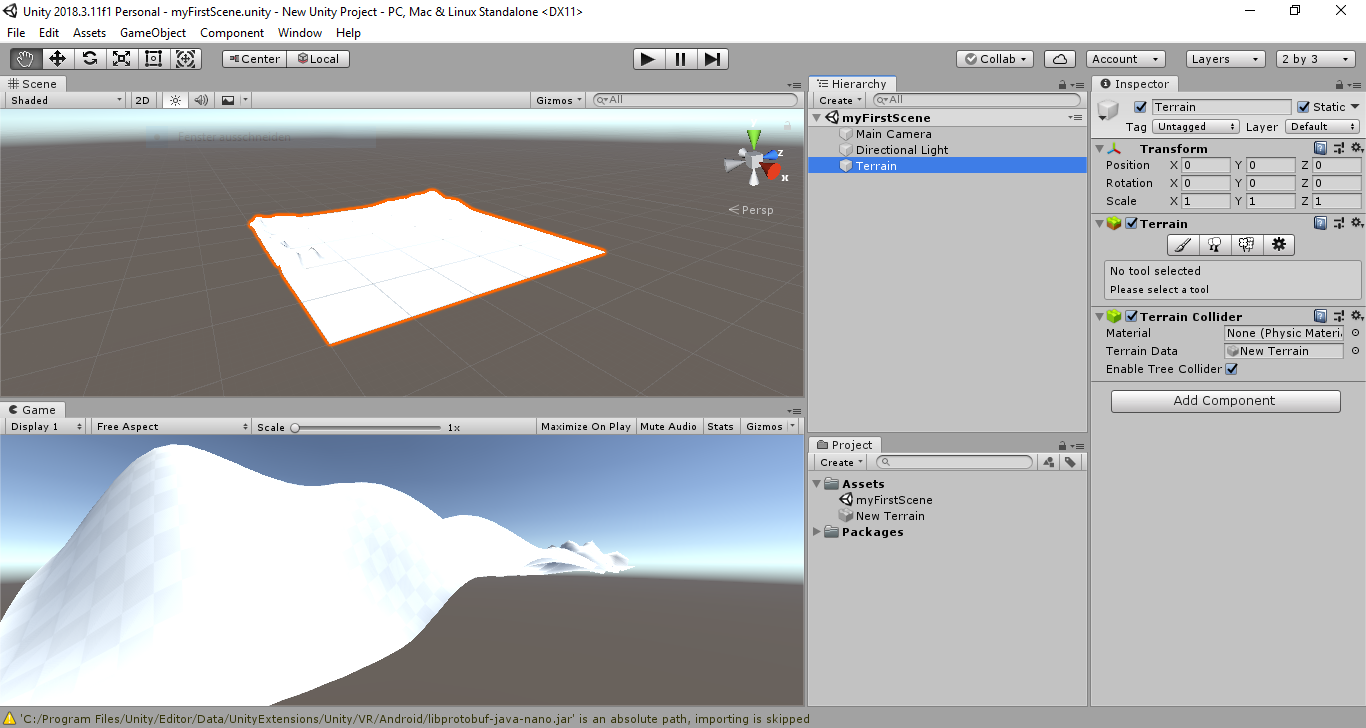
\includegraphics[width=16cm]{kapitel/editor.PNG}
  \centering
  \caption{Screenshot of Unity editor}
  \label{fig:unity-editor}
\end{figure}
\subsection{Scripting in Unity}
\subsection{Unity and Samsung Gear VR support}
In Unity, VR support can simply be enabled by ticking a box in the player settings. However, to make a game work together with the Samsung Gear VR, more work than that has to be done. First of all, the Occulus support library has to be imported.
\section{Environment design of different scenes}
\section{VR specific problems}
\subsection{Input methods with Samsung Gear VR controller}
\subsection{Implementation of the dialog system}